\documentclass{article}
\usepackage[utf8]{inputenc}
\usepackage[icelandic]{babel}
\usepackage[T1]{fontenc}
\usepackage{graphicx}
\usepackage{mathtools}
\usepackage{amsmath}
\usepackage{amssymb}
\usepackage{minted}


\graphicspath{ {./imgs} }
\title{Titill - Áfangi}
\author{ttb3@hi.is}
\date{\today}


\begin{document}
\maketitle


\section*{1. Um hvað snérist verkefnið}
Verkefnið snérist um að útbúa rafrás sem gat tekið inn merki á BCD kóðaformi, breytt því merki yfir í Excess-3 kóðaform og skilað nýja merkinu.
Til að gera verkefnið þurfti að nota nokkrar tæknir sem er búið að kenna eins og að, skrifa inn í og lesa úr k-kortum og breyta úr SOP-boolean rás yfir í NAND-rás.

\section*{2. Hvað gerði ég?}

Ég byrjaði á því að krota upp grófa sanntöflu fyrir rásina, reikna með öllum inntökum og merki þau sem á ekki að taka með í reikninginn sem x.
\begin{center}
    \begin{tabular}{|c|c|c|c|c|c|c|c|c|c|}
        \hline
        out&ignore&B0&B1&B2&B3&E0&E1&E2&E3\\
        \hline
        0 & &0&0&0&0&0&0&1&1\\
        \hline
        1 & &0&0&0&1&0&1&0&0\\
        \hline
        2 & &0&0&1&0&0&1&0&1\\
        \hline
        3 & &0&0&1&1&0&1&1&0\\
        \hline
        4 & &0&1&0&0&0&1&1&1\\
        \hline
        5 & &0&1&0&1&1&0&0&0\\
        \hline
        6 & &0&1&1&0&1&0&0&1\\
        \hline
        7 & &0&1&1&1&1&0&1&0\\
        \hline
        8 & &1&0&0&0&1&0&1&1\\
        \hline
        9 & &1&0&0&1&1&1&0&0\\
        \hline
        10&x&1&0&1&0&x&x&x&x\\
        \hline
        11&x&1&0&1&1&x&x&x&x\\
        \hline
        12&x&1&1&0&0&x&x&x&x\\
        \hline
        13&x&1&1&0&1&x&x&x&x\\
        \hline
        14&x&1&1&1&0&x&x&x&x\\
        \hline
        15&x&1&1&1&1&x&x&x&x\\
        \hline
    \end{tabular}
\end{center}

Útfrá sanntöflunni bjó ég svo til k-kort til að fá betri yfirsýn yfir það hvernig rásin myndi að lokum líta út.

\begin{center}
    \begin{tabular}{|c|c|c|c|c|c|}
        \hline
        &&CD&CD&CD&CD\\
        \hline
        &&00&01&11&10\\
        \hline
        AB&00&0&0&0&0\\
        \hline
        AB&01&0&1&1&1\\
        \hline
        AB&11&1&1&x&x\\
        \hline
        AB&10&x&x&x&x\\
        \hline
    \end{tabular}
\end{center}

Ég tók svo fjögur af þessu k-korti, eitt fyrir hvert output í excess-3, og bjó til SOP-boolean jöfnu fyrir hvert og eitt. 
Þessi kort og jöfnur hvers og eins má sjá hér fyrir neðan, reitir sem tengdir eru saman eru litaðir í sama lit og ef reitur er notaður oftar en einu sinni, 
ætti að vera í nokkrum litum, þá reyndi ég að afmarka hann með þykkari border línu.

\begin{center}
    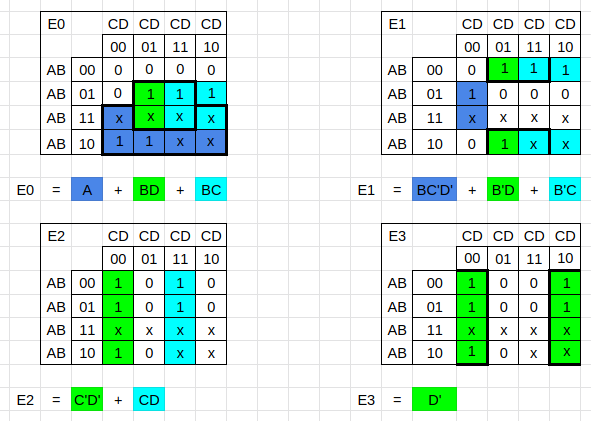
\includegraphics[scale=0.5]{kkort.png}
\end{center}

Núna er ég kominn með boolean jöfnu fyrir hvert output á XS-3 formi:
\begin{align*}
    E0=&A+BD+BC\\
    E1=&BC'D'+B'D+B'C\\
    E2=&C'D'+CD\\
    E3=&D'
\end{align*}
Þá er auðvelt að búa til rásir fyrir hvert output, sjá fyrir neðan:
\begin{center}
    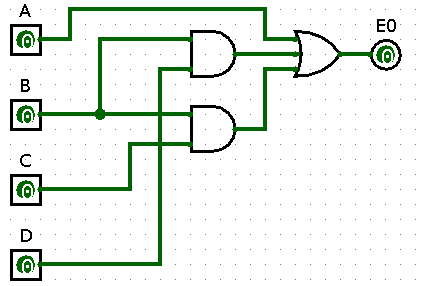
\includegraphics[scale=0.2]{sc1.png}
    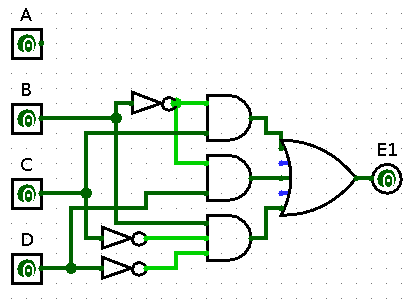
\includegraphics[scale=0.2]{sc2.png}
    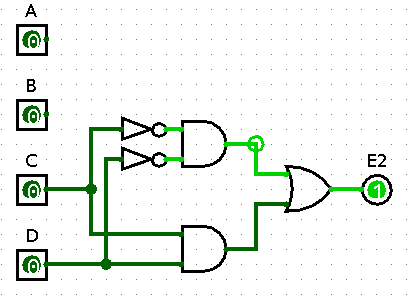
\includegraphics[scale=0.2]{sc4.png}
    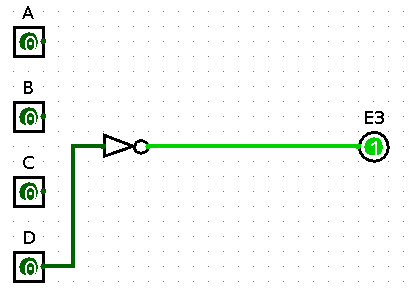
\includegraphics[scale=0.2]{sc3.png}
\end{center}
\newpage

Þá er næsta skref að breyta þessum rásum í NAND rásir, sjá fyrir neðan:
\begin{center}
    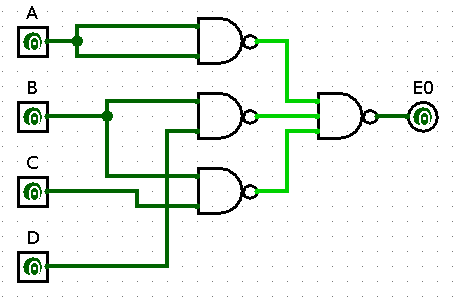
\includegraphics[scale=0.25]{nand0.png}
    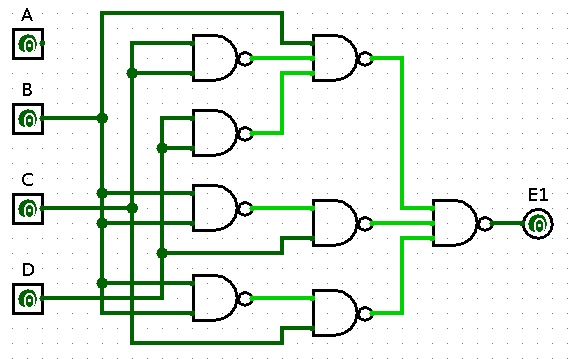
\includegraphics[scale=0.25]{nand1.png}
    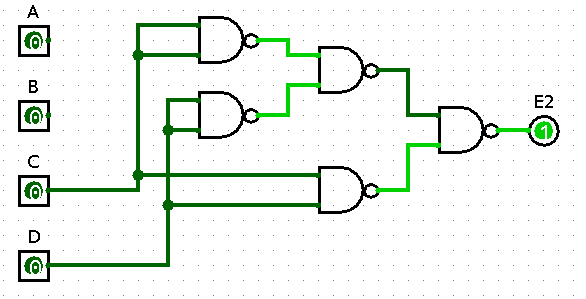
\includegraphics[scale=0.25]{nand2.png}
    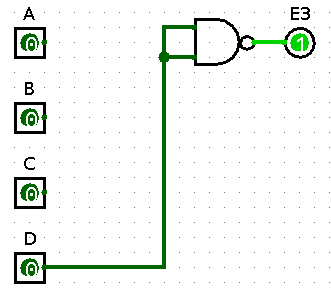
\includegraphics[scale=0.25]{nand3.png}
\end{center}

Þá var aðeins að fegra aðeins upp á rásirnar og tengja þær svo allar saman og fá þá út þessa rás:
\begin{center}
    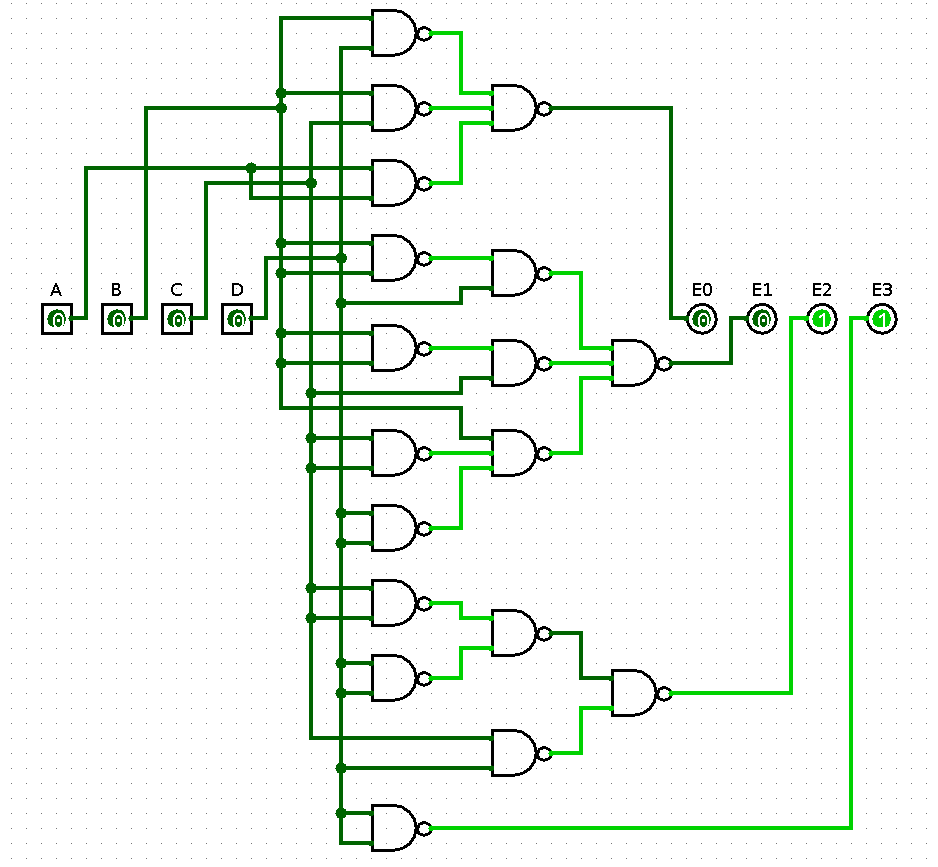
\includegraphics[scale=0.35]{heil.png}
    Rásin með öll input 0

    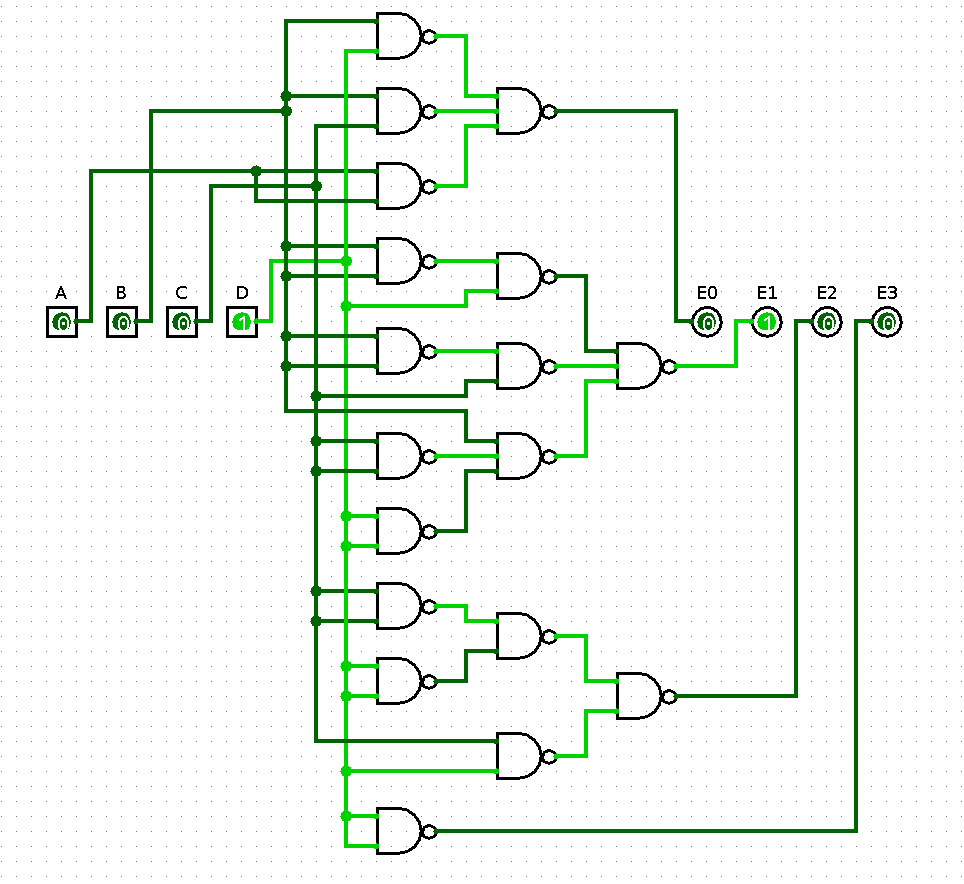
\includegraphics[scale=0.35]{heil2.png}
    Rásin með input 0001

    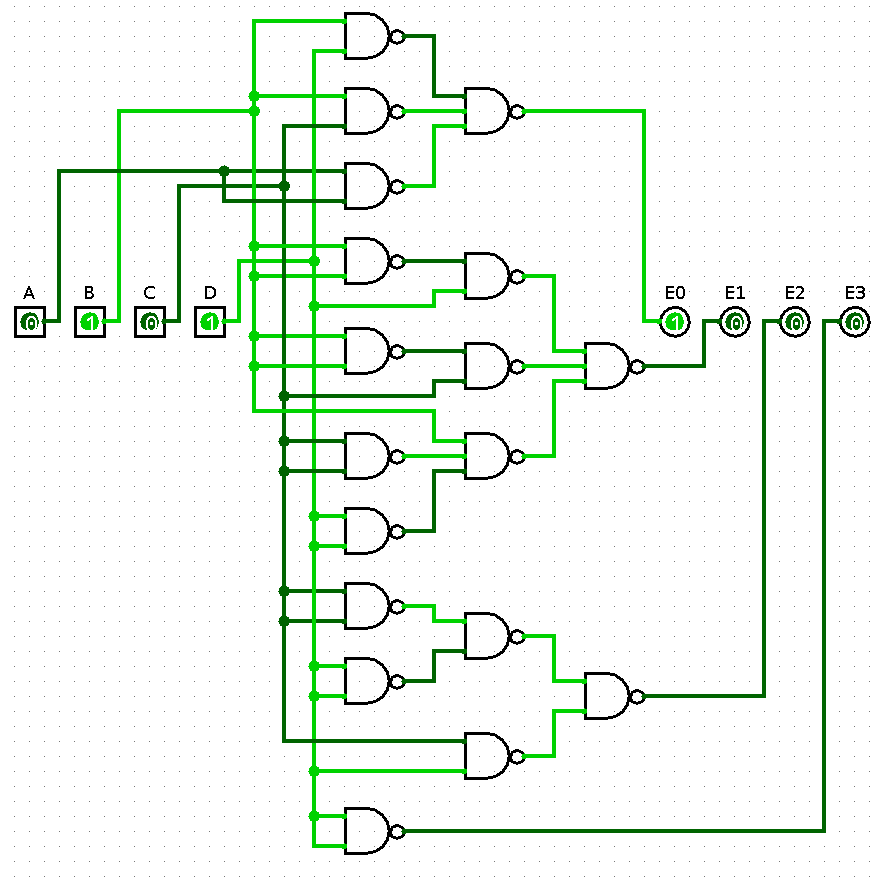
\includegraphics[scale=0.37]{heil3.png}
    Rásin með input 0101
\end{center}

\section*{3. Hvernig gekk?}
Verkefnið þegar á heildina er litið gekk frekar vel, ég þurfti að lesa mér aðeins meira til um K-kort en eftir að vera kominn með góðann skilning
á þeim gekk allt smurt fyrir sig.

\newpage
\section*{4. Niðurstöður}
Ég prófaði rásina fyrir öll gildi í sanntöflunni og til minnar ánægju var útkoman alltaf rétt.
sjá næstu töflu, sem forritið bjó til fyrir mig:
\begin{center}
    \begin{tabular}{|c|c|c|c|c|c|c|c|}
        \hline
        A&	B&	C&	D&	E0&	E1&	E2&	E3\\
        \hline
        0&	0&	0&	0&	0&	0&	1&	1\\
        \hline
        0&	0&	0&	1&	0&	1&	0&	0\\
        \hline
        0&	0&	1&	0&	0&	1&	0&	1\\
        \hline
        0&	0&	1&	1&	0&	1&	1&	0\\
        \hline
        0&	1&	0&	0&	0&	1&	1&	1\\
        \hline
        0&	1&	0&	1&	1&	0&	0&	0\\
        \hline
        0&	1&	1&	0&	1&	0&	0&	1\\
        \hline
        0&	1&	1&	1&	1&	0&	1&	0\\
        \hline
        1&	0&	0&	0&	1&	0&	1&	1\\
        \hline
        1&	0&	0&	1&	1&	1&	0&	0\\
        \hline
    \end{tabular}
\end{center}

\end{document}